\begin{figure}
  \centering
  \begin{adjustbox}{width=.7\linewidth,center}
    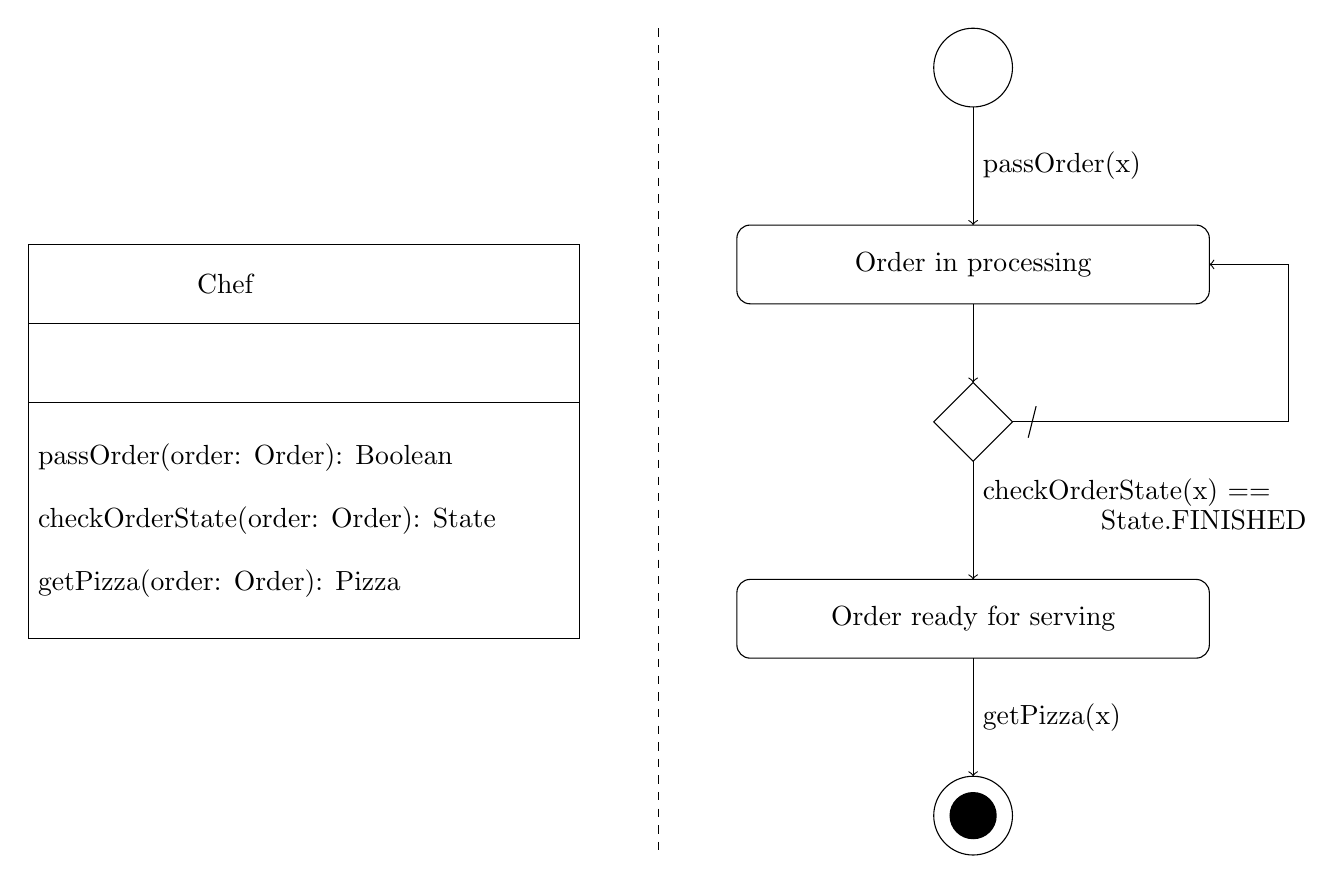
\begin{tikzpicture}
      \draw[dashed] (0,5) -- (0,-5.5);

      \begin{scope}[shift={(0,-0.25)}]
        \draw (-8,2.5) rectangle (-1,-2.5);
        \draw (-8,1.5) -- (-1,1.5);
        \draw (-8,0.5) -- (-1,0.5);
        \draw (-5.5,2) node{Chef};
        \draw (-8,-0.2) node[anchor=west] {passOrder(order: Order): Boolean};
        \draw (-8,-1) node[anchor=west] {checkOrderState(order: Order): State};
        \draw (-8,-1.8) node[anchor=west] {getPizza(order: Order): Pizza};
      \end{scope}

      \draw (4, 4.5) circle[radius=0.5];
      \draw[->] (4,4) -- (4,2.5);
      \draw (4,3.25) node[anchor=west] {passOrder(x)};
      \draw[rounded corners=4.8pt] (1,2.5) rectangle (7,1.5);
      \draw (4,2) node {Order in processing};
      \draw[->] (4,1.5) -- (4,0.5);
      \draw (4,0.5) -- (4.5,0) -- (4,-0.5) -- (3.5,0) -- cycle;
      \draw[->] (4.5,0) -- (8,0)-- (8,2) -- (7,2);
      \draw (4.7,-0.2) -- (4.8,0.2);
      \draw[->] (4,-0.5) -- (4,-2);
      \draw (4,-0.9) node[anchor=west] {checkOrderState(x) ==};
      \draw (5.5,-1) node[anchor=north west] {State.FINISHED};
      \draw[rounded corners=4.8pt] (1,-3) rectangle (7,-2);
      \draw (4,-2.5) node {Order ready for serving};
      \draw[->] (4,-3) -- (4,-4.5);
      \draw (4,-3.75) node[anchor=west] {getPizza(x)};
      \draw (4, -5) circle[radius=0.5];
      \fill (4, -5) circle[radius=0.3];
    \end{tikzpicture}
  \end{adjustbox}
\end{figure}
